\subsection{Interface Signals}
\label{sec:is}

The interface signals of the Versat controller core are described in Table~\ref{tab:is}.

\begin{table}[h]
\centering
\begin{tabular}{|l|c|l|}
\hline
\multicolumn{1}{|c|}{\bf Name} & {\bf Direction} & \multicolumn{1}{c|}{\bf Description}                                                     \\ \hline \hline
\multicolumn{1}{|l|}{clk}                                & IN              & Clock signal.                                                  \\ \hline
\multicolumn{1}{|l|}{rst}                                & IN              & \multicolumn{1}{l|}{Reset signal.}                             \\ \hline \hline
\multicolumn{3}{|c|}{{\bf Instruction Interface}}                                                                                           \\ \hline \hline
instruction{[}7:0{]}                                     & IN              & Instruction to execute.                                        \\ \hline
pc{[}9:0{]}                                              & OUT             & Program Counter.                                               \\ \hline \hline
\multicolumn{3}{|c|}{{\bf RW Bus Interface}}                                                                                                \\ \hline \hline
rw\_req                                                  & OUT             & Data request for read or write.                                \\ \hline
rw\_rnw                                                  & OUT             & Data read (1) or write (0) signal.                             \\ \hline
rw\_addr{[}9:0{]}                                        & OUT             & Data address.                                                  \\ \hline
rw\_data\_to\_rd{[}7:0{]}                                & IN              & Data to read.                                                  \\ \hline
rw\_data\_to\_wr{[}7:0{]}                                & OUT             & Data to write.                                                 \\ \hline
\end{tabular}
\caption{Interface signals.}
\label{tab:is}
\end{table}

\subsubsection{Instruction Interface Timing Diagram}
\label{sec:instrird}

The timing diagram for pipelined instruction read using the
Instruction Interface is shown in Figure~\ref{fig:instrird}.

\begin{figure}[htbp]
    \centerline{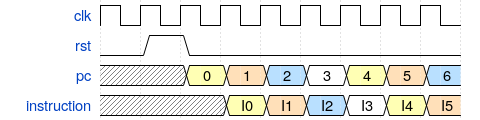
\includegraphics[width=.8\textwidth]{instr_rd}}
    \vspace{0cm}\caption{Instruction interface pipelined reads.}
    \label{fig:instrird}
\end{figure}

\subsubsection{RW Bus Interface Timing Diagram}
\label{sec:rwi}

The timing diagrams for reads and writes using the RW Bus Interface
are shown in Figure~\ref{fig:rwird} and Figure~\ref{fig:rwiwr},
respectively. These operations may be consecutive or not, as
illustrated.

\begin{figure}[htbp]
    \centerline{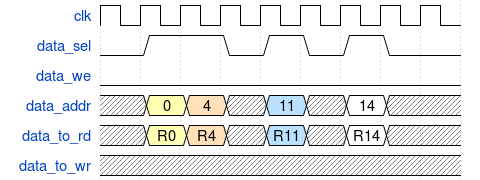
\includegraphics[width=.8\textwidth]{rw_rd}}
    \vspace{0cm}\caption{RW bus interface reads.}
    \label{fig:rwird}
\end{figure}

\begin{figure}[htbp]
    \centerline{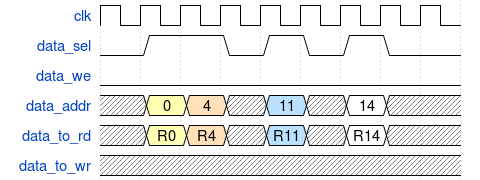
\includegraphics[width=.8\textwidth]{rw_wr}}
    \vspace{0cm}\caption{RW bus interface writes.}
    \label{fig:rwiwr}
\end{figure}

